\documentclass[class=article, crop=false]{standalone}
%\documentclass[12pt]{article}
\usepackage{tikz}
\usepackage{subcaption}
\usetikzlibrary{calc}
\usetikzlibrary {shapes.geometric}

\begin{document}
\begin{figure}
    \centering
    % Row 1
    \begin{minipage}{0.16\textwidth}
        \centering
        \scalebox{0.8}{\documentclass[class=article, crop=false]{standalone}
\usepackage{tikz}
\usepackage{subcaption}
\usetikzlibrary{calc}

\begin{document}
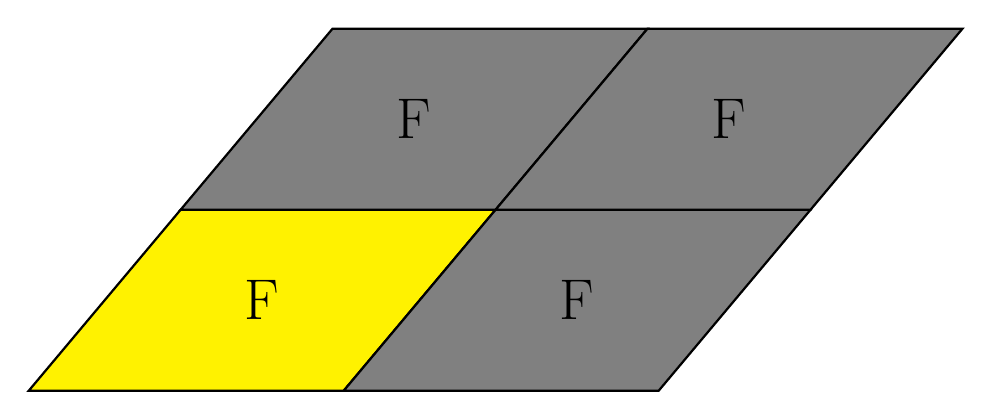
\begin{tikzpicture}
    % Define the lengths of the sides and the angle
    \def\a{4}  % length of side a
    \def\b{3}  % length of side b
    \def\angle{50}  % angle between sides a and b
    \def\s{F} % Label in center of cells

    % Calculate the coordinates of the points
    \coordinate (C00) at (0, 0);
    \coordinate (C10) at (\a, 0);
    \coordinate (C11) at ({\a + \b*cos(\angle)}, {\b * sin(\angle)});
    \coordinate (C01) at ({\b * cos(\angle)}, {\b * sin(\angle)});
    \coordinate (C02) at ({2*\b*cos(\angle)}, {2*\b * sin(\angle)});
    \coordinate (C12) at ({\a +2*\b * cos(\angle)}, {2*\b * sin(\angle)});
    \coordinate (C22) at ({2*\a + 2*\b * cos(\angle)}, {2*\b * sin(\angle)});
    \coordinate (C21) at ({2*\a + \b*cos(\angle)}, {\b * sin(\angle)});
    \coordinate (C20) at ({2*\a}, 0);

        
    % Draw the oblique unit cell
    \draw[thick,fill=yellow] (C00) -- (C10) -- (C11) -- (C01) -- cycle;
    \draw[thick,fill=gray] (C01) -- (C11) -- (C12) -- (C02) -- cycle;
    \draw[thick,fill=gray] (C10) -- (C20) -- (C21) -- (C11) -- cycle;
    \draw[thick,fill=gray] (C11) -- (C21) -- (C22) -- (C12) -- cycle;

    % Center symbols
    \node at ($(C00)!0.5!(C11)$) {\huge \s};
    \node at ($(C20)!0.5!(C11)$) {\huge \s};
    \node at ($(C02)!0.5!(C11)$) {\huge \s};
    \node at ($(C22)!0.5!(C11)$) {\huge \s};
\end{tikzpicture}
\end{document}}
        \caption{p1}
    \end{minipage}
    \hfill
    \begin{minipage}{0.16\textwidth}
        \centering
        \scalebox{0.8}{\documentclass[class=article, crop=false]{standalone}
\usepackage{tikz}
\usepackage{subcaption}
\usetikzlibrary{calc}
\usetikzlibrary {shapes.geometric}

\begin{document}
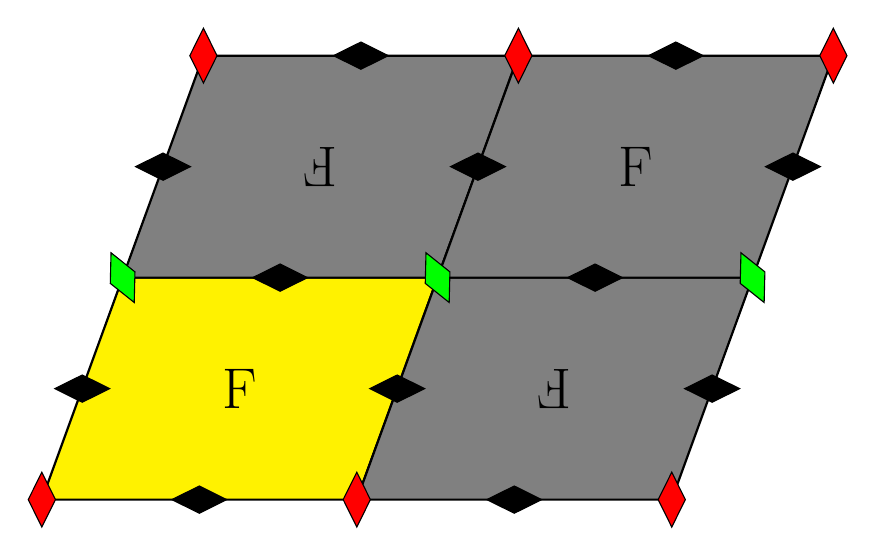
\begin{tikzpicture}
    % Define the lengths of the sides and the angle
    \def\a{4}  % length of side a
    \def\b{3}  % length of side b
    \def\angle{70}  % angle between sides a and b
    \def\s{F} % Label in center of cells

    % Calculate the coordinates of the points
    \coordinate (C00) at (0, 0);
    \coordinate (C10) at (\a, 0);
    \coordinate (C11) at ({\a + \b*cos(\angle)}, {\b * sin(\angle)});
    \coordinate (C01) at ({\b * cos(\angle)}, {\b * sin(\angle)});
    \coordinate (C02) at ({2*\b*cos(\angle)}, {2*\b * sin(\angle)});
    \coordinate (C12) at ({\a +2*\b * cos(\angle)}, {2*\b * sin(\angle)});
    \coordinate (C22) at ({2*\a + 2*\b * cos(\angle)}, {2*\b * sin(\angle)});
    \coordinate (C21) at ({2*\a + \b*cos(\angle)}, {\b * sin(\angle)});
    \coordinate (C20) at ({2*\a}, 0);
        
    % Draw the oblique unit cell
    \draw[thick,fill=yellow] (C00) -- (C10) -- (C11) -- (C01) -- cycle;
    \draw[thick,fill=gray] (C10) -- (C20) -- (C21) -- (C11) -- cycle;
    \draw[thick,fill=gray] (C01) -- (C11) -- (C12) -- (C02) -- cycle;
    \draw[thick,fill=gray] (C11) -- (C21) -- (C22) -- (C12) -- cycle;
    
    % Draw chiral center
    \node at ($(C00)!0.5!(C11)$) {\huge \s};
    \node[rotate=180] at ($(C01)!0.5!(C12)$) {\huge \s};
    \node at ($(C11)!0.5!(C22)$) {\huge \s};
    \node[rotate=180] at ($(C10)!0.5!(C21)$) {\huge \s};

    % Draw node reflections
    \draw (C00)  node[shape aspect=0.5,diamond,draw,fill=red] {};
    \draw (C10)  node[shape aspect=0.5,diamond,draw,fill=red] {};
    \draw (C20)  node[shape aspect=0.5,diamond,draw,fill=red] {};
    \draw (C01)  node[rotate = \angle-45,shape aspect=0.5,diamond,draw,fill=green] {};
    \draw (C11)  node[rotate = \angle-45,shape aspect=0.5,diamond,draw,fill=green] {};
    \draw (C21)  node[rotate = \angle-45,shape aspect=0.5,diamond,draw,fill=green] {};
    \draw (C02)  node[shape aspect=0.5,diamond,draw,fill=red] {};
    \draw (C12)  node[shape aspect=0.5,diamond,draw,fill=red] {};
    \draw (C22)  node[shape aspect=0.5,diamond,draw,fill=red] {}; 
    \draw ($(C00)!0.5!(C10)$)  node[rotate=90,shape aspect=0.5,diamond,draw,fill=black] {};
    \draw ($(C10)!0.5!(C20)$)  node[rotate=90,shape aspect=0.5,diamond,draw,fill=black] {};
    \draw ($(C00)!0.5!(C01)$)  node[rotate=90,shape aspect=0.5,diamond,draw,fill=black] {};
    \draw ($(C10)!0.5!(C11)$)  node[rotate=90,shape aspect=0.5,diamond,draw,fill=black] {};
    \draw ($(C20)!0.5!(C21)$)  node[rotate=90,shape aspect=0.5,diamond,draw,fill=black] {};
    \draw ($(C01)!0.5!(C02)$)  node[rotate=90,shape aspect=0.5,diamond,draw,fill=black] {};
    
    \draw ($(C01)!0.5!(C11)$)  node[rotate=90,shape aspect=0.5,diamond,draw,fill=black] {};
    \draw ($(C11)!0.5!(C21)$)  node[rotate=90,shape aspect=0.5,diamond,draw,fill=black] {};
    
    \draw ($(C11)!0.5!(C12)$)  node[rotate=90,shape aspect=0.5,diamond,draw,fill=black] {};
    \draw ($(C21)!0.5!(C22)$)  node[rotate=90,shape aspect=0.5,diamond,draw,fill=black] {};
    \draw ($(C02)!0.5!(C12)$)  node[rotate=90,shape aspect=0.5,diamond,draw,fill=black] {};
    \draw ($(C12)!0.5!(C22)$)  node[rotate=90,shape aspect=0.5,diamond,draw,fill=black] {};
\end{tikzpicture}
\end{document}}
        \caption{p2}
    \end{minipage}
    \hfill
    % Row 2
    \begin{minipage}{0.16\textwidth}
        \centering
        \scalebox{0.8}{\documentclass[class=article, crop=false]{standalone}
\usepackage{tikz}
\usepackage{subcaption}
\usetikzlibrary{calc}
\usetikzlibrary {shapes.geometric}

\begin{document}
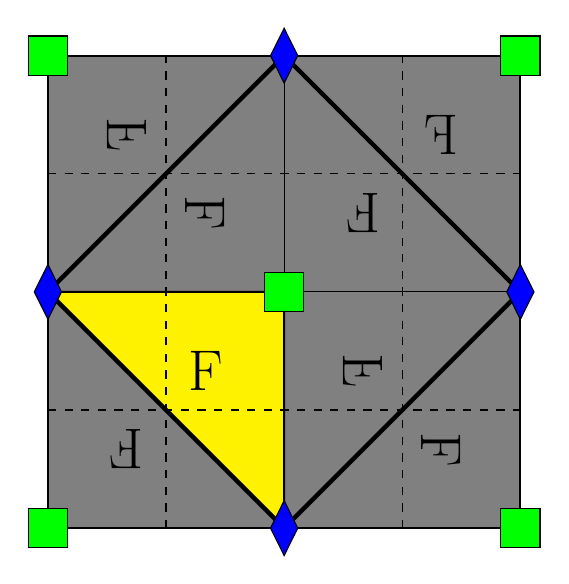
\begin{tikzpicture}
            % Define the lengths of the sides and the angle
            \def\a{3}  % length of side a
            \def\b{3}  % length of side b
            \def\angle{90}  % angle between sides a and b
            \def\s{F}
        
            % Calculate the coordinates of the points
            \coordinate (C00) at (0, 0);
            \coordinate (C10) at (\a, 0);
            \coordinate (C11) at ({\a + \b*cos(\angle)}, {\b * sin(\angle)});
            \coordinate (C01) at ({\b * cos(\angle)}, {\b * sin(\angle)});
            \coordinate (C02) at ({2*\b*cos(\angle)}, {2*\b * sin(\angle)});
            \coordinate (C12) at ({\a +2*\b * cos(\angle)}, {2*\b * sin(\angle)});
            \coordinate (C22) at ({2*\a + 2*\b * cos(\angle)}, {2*\b * sin(\angle)});
            \coordinate (C21) at ({2*\a + \b*cos(\angle)}, {\b * sin(\angle)});
            \coordinate (C20) at ({2*\a}, 0);
        
            % Draw the oblique unit cell
            \draw[thick,fill=gray] (C00) -- (C20) -- (C22) -- (C02) -- cycle;
            \draw[thick,fill=yellow] (C01) -- (C10) -- (C11) -- cycle;
            \draw[ultra thick] (C10) -- (C21) -- (C12) -- (C01) -- cycle;

            
            % Draw mirrow lines
            \draw[dashed] ($(C00)!0.5!(C10)$) -- ($(C02)!0.5!(C12)$);
            \draw[thin] (C10) -- (C12);
            \draw[dashed] ($(C10)!0.5!(C20)$) -- ($(C12)!0.5!(C22)$);
            \draw[dashed] ($(C00)!0.5!(C01)$) -- ($(C20)!0.5!(C21)$);
            \draw[thin] (C01) -- (C21);
            \draw[dashed] ($(C01)!0.5!(C02)$) -- ($(C21)!0.5!(C22)$);
            
            % Draw chiral center
            \node[rotate=180] at ($(C11)!0.6666!(C00)$) {\huge \s};
            \node at ($(C11)!0.3333!(C00)$) {\huge \s};
            \node[rotate=90] at ($(C11)!0.6666!(C02)$) {\reflectbox{\huge \s}};
            \node[rotate=-90] at ($(C11)!0.3333!(C02)$) {\huge \s};
            \node at ($(C11)!0.6666!(C22)$) {\reflectbox{\huge \s}};
            \node[rotate=180] at ($(C11)!0.3333!(C22)$) {\huge \s};
            \node[rotate=-90] at ($(C11)!0.6666!(C20)$) {\huge \s};
            \node[rotate=90] at ($(C11)!0.3333!(C20)$) {\reflectbox{\huge 
            \s}};

            % Draw node reflections
            \draw (C00)  node[minimum size=0.5cm,draw,fill=green] {};
            \draw (C10)  node[shape aspect=0.5,diamond,draw,fill=blue] {};
            \draw (C11)  node[minimum size=0.5cm,draw,fill=green] {};
            \draw (C01)  node[shape aspect=0.5,diamond,draw,fill=blue] {};
            \draw (C02)  node[minimum size=0.5cm,draw,fill=green] {};
            \draw (C12)  node[shape aspect=0.5,diamond,draw,fill=blue] {};
            \draw (C22)  node[minimum size=0.5cm,draw,fill=green] {};
            \draw (C21)  node[shape aspect=0.5,diamond,draw,fill=blue] {};
            \draw (C20)  node[minimum size=0.5cm,draw,fill=green] {};

            %\draw ($(A)!0.5!(E)$) node[shape aspect=0.5,diamond,draw,fill=black] {};
            
        \end{tikzpicture}
\end{document}}
        \caption{p4g}
    \end{minipage}
    \hfill
    \begin{minipage}{0.16\textwidth}
        \centering
        \scalebox{0.8}{\documentclass[class=article, crop=false]{standalone}
\usepackage{tikz}
\usepackage{subcaption}
\usetikzlibrary{calc}
\usetikzlibrary {shapes.geometric}

\begin{document}
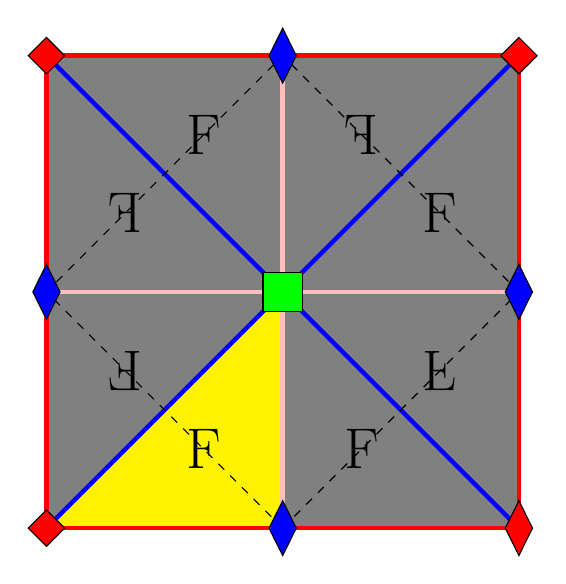
\begin{tikzpicture}
            % Define the lengths of the sides and the angle
            \def\a{3}  % length of side a
            \def\b{3}  % length of side b
            \def\angle{90}  % angle between sides a and b
            \def\s{F}
        
            % Calculate the coordinates of the points
            \coordinate (C00) at (0, 0);
            \coordinate (C10) at (\a, 0);
            \coordinate (C11) at ({\a + \b*cos(\angle)}, {\b * sin(\angle)});
            \coordinate (C01) at ({\b * cos(\angle)}, {\b * sin(\angle)});
            \coordinate (C02) at ({2*\b*cos(\angle)}, {2*\b * sin(\angle)});
            \coordinate (C12) at ({\a +2*\b * cos(\angle)}, {2*\b * sin(\angle)});
            \coordinate (C22) at ({2*\a + 2*\b * cos(\angle)}, {2*\b * sin(\angle)});
            \coordinate (C21) at ({2*\a + \b*cos(\angle)}, {\b * sin(\angle)});
            \coordinate (C20) at ({2*\a}, 0);
        
            % Draw the oblique unit cell
            \draw[thick,fill=gray] (C00) -- (C20) -- (C22) -- (C02) -- cycle;
            \draw[thick,fill=yellow] (C00) -- (C10) -- (C11) -- cycle;
            \draw[ultra thick,red] (C00) -- (C20) -- (C22) -- (C02) -- cycle;
            \draw[ultra thick,blue] (C11) -- (C00);
            \draw[ultra thick,blue] (C11) -- (C20);
            \draw[ultra thick,blue] (C11) -- (C22);
            \draw[ultra thick,blue] (C11) -- (C02);
            \draw[ultra thick,pink] (C11) -- (C10);
            \draw[ultra thick,pink] (C11) -- (C21);
            \draw[ultra thick,pink] (C11) -- (C12);
            \draw[ultra thick,pink] (C11) -- (C01);
            
            % Draw mirrow lines
            \draw[dashed] (C10) -- (C21) -- (C12) -- (C01) -- cycle;
            
            % Draw chiral center
            \node at ($(C01)!0.6666!(C10)$) {\huge \s};
            \node[rotate=180] at ($(C01)!0.3333!(C10)$) {\huge \s};
            \node[rotate=180] at ($(C10)!0.6666!(C21)$) {\reflectbox{\huge \s}};
            \node at ($(C10)!0.3333!(C21)$) {\huge \s};
            \node at ($(C21)!0.6666!(C12)$) {\reflectbox{\huge \s}};
            \node at ($(C21)!0.3333!(C12)$) {\huge \s};
            \node at ($(C01)!0.6666!(C12)$) {\huge \s};
            \node[rotate=0] at ($(C01)!0.3333!(C12)$) {\reflectbox{\huge \s}};

            % Draw node reflections
            \draw (C00)  node[shape aspect=1,diamond,draw,fill=red] {};
            \draw (C10)  node[shape aspect=0.5,diamond,draw,fill=blue] {};
            \draw (C11)  node[minimum size=0.5cm,draw,fill=green] {};
            \draw (C01)  node[shape aspect=0.5,diamond,draw,fill=blue] {};
            \draw (C02)  node[shape aspect=1,diamond,draw,fill=red] {};
            \draw (C12)  node[shape aspect=0.5,diamond,draw,fill=blue] {};
            \draw (C22)  node[shape aspect=1,diamond,draw,fill=red] {};
            \draw (C21)  node[shape aspect=0.5,diamond,draw,fill=blue] {};
            \draw (C20)  node[shape aspect=0.5,diamond,draw,fill=red] {};

            %\draw ($(A)!0.5!(E)$) node[shape aspect=0.5,diamond,draw,fill=black] {};
            
        \end{tikzpicture}
\end{document}}
        \caption{p4m}
    \end{minipage}
    % Row 3
    \vfill
    \begin{minipage}{0.16\textwidth}
        \centering
        \scalebox{0.8}{\documentclass[class=article, crop=false]{standalone}
\usepackage{tikz}
\usepackage{subcaption}
\usetikzlibrary{calc}
\usetikzlibrary {shapes.geometric}

\begin{document}
\begin{tikzpicture}
            % Define the lengths of the sides and the angle
            \def\a{3}  % length of side a
            \def\b{3}  % length of side b
            \def\angle{60}  % angle between sides a and b
            \def\s{F} % Label in center of cells
        
            % Calculate the coordinates of the points
            \coordinate (C00) at (0, 0);
            \coordinate (C10) at (\a, 0);
            \coordinate (C11) at ({\a + \b*cos(\angle)}, {\b * sin(\angle)});
            \coordinate (C01) at ({\b * cos(\angle)}, {\b * sin(\angle)});
            \coordinate (C02) at ({2*\b*cos(\angle)}, {2*\b * sin(\angle)});
            \coordinate (C12) at ({\a +2*\b * cos(\angle)}, {2*\b * sin(\angle)});
            \coordinate (C22) at ({2*\a + 2*\b * cos(\angle)}, {2*\b * sin(\angle)});
            \coordinate (C21) at ({2*\a + \b*cos(\angle)}, {\b * sin(\angle)});
            \coordinate (C20) at ({2*\a}, 0);

            \coordinate (A1) at ($(C00)!0.6666!(C11)$);
            \coordinate (A2) at ($(C11)!0.3333!(C22)$);
        
            % Draw the oblique unit cell
            \draw[thick,fill=gray] (C00) -- (C20) -- (C22) -- (C02) -- cycle;
            \draw[thick,fill=yellow] (C00) -- (A1) -- (C20) -- cycle;
            %\draw[thick] (C10) -- (C21) -- (C12) -- (C01) -- cycle;
            
            % Draw mirrow lines
            \draw[thin] (C02) -- (A1);
            \draw[thin] (C02) -- (C11) -- (C20);
            \draw[thin] (C02) -- (A2) -- (C20);
            \draw[thin] (A2) -- (C22);
            
            % Draw chiral center
            $\node at ($(C00)!0.5!(C20)!0.5!(A1)$) {\huge \s};
            \node[rotate=240] at ($(C00)!0.5!(C02)!0.5!(A1)$) {\huge \s};
            \node[rotate=120] at ($(C20)!0.5!(C02)!0.5!(A1)$) {\huge \s};
            \node[rotate=300] at ($(C20)!0.5!(C02)!0.5!(A2)$) {\huge \s};
            \node[rotate=60] at ($(C22)!0.5!(C20)!0.5!(A2)$) {\huge \s};
            \node[rotate=180] at ($(C02)!0.5!(C22)!0.5!(A2)$) {\huge \s};

            % Draw node rotations
            \draw (C00)  node[regular polygon, regular polygon sides=6, draw, fill=blue, minimum size=0.5cm] {};
            \draw (C10)  node[shape aspect=0.5,diamond,draw,fill=black] {};
            \draw (C21)  node[shape aspect=0.5,diamond,draw,fill=black] {};
            \draw (C01)  node[shape aspect=0.5,diamond,draw,fill=black] {};
            \draw (C12)  node[shape aspect=0.5,diamond,draw,fill=black] {};
            \draw (C02)  node[regular polygon, regular polygon sides=6, draw, fill=blue, minimum size=0.5cm] {};
            %\draw (C12)  node[shape aspect=0.5,rotate=90,diamond,draw,fill=blue] {};
            \draw (C22)  node[regular polygon, regular polygon sides=6, draw, fill=blue, minimum size=0.5cm] {};
            %\draw (C21)  node[shape aspect=0.5,rotate=90,diamond,draw,fill=blue] {};
            \draw (C20)  node[regular polygon, regular polygon sides=6, draw, fill=blue, minimum size=0.5cm] {};

            \draw (A1)  node[regular polygon, regular polygon sides=3, draw, fill=red, minimum size=0.5cm] {};
            \draw (A2)  node[regular polygon, regular polygon sides=3, draw, fill=red, minimum size=0.5cm] {};

            \draw (C11) node[shape aspect=0.5,diamond,draw,fill=black] {};
            
        \end{tikzpicture}
\end{document}}
        \caption{p6}
    \end{minipage}
    \hfill
    \begin{minipage}{0.16\textwidth}
        \centering
        \scalebox{0.8}{\documentclass[class=article, crop=false]{standalone}
\usepackage{tikz}
\usepackage{subcaption}
\usetikzlibrary{calc}
\usetikzlibrary {shapes.geometric}

\begin{document}
\begin{tikzpicture}
    % Define the lengths of the sides and the angle
    \def\a{3}  % length of side a
    \def\b{3}  % length of side b
    \def\angle{60}  % angle between sides a and b
    \def\s{T} % Label in center of cells

    % Calculate the coordinates of the points
    \coordinate (C00) at (0, 0);
g10) at (\a, 0);
    \coordinate (C11) at ({\a + \b*cos(\angle)}, {\b * sin(\angle)});
    \coordinate (C01) at ({\b * cos(\angle)}, {\b * sin(\angle)});
    \coordinate (C02) at ({2*\b*cos(\angle)}, {2*\b * sin(\angle)});
    \coordinate (C12) at ({\a +2*\b * cos(\angle)}, {2*\b * sin(\angle)});
    \coordinate (C22) at ({2*\a + 2*\b * cos(\angle)}, {2*\b * sin(\angle)});
    \coordinate (C21) at ({2*\a + \b*cos(\angle)}, {\b * sin(\angle)});
    \coordinate (C20) at ({2*\a}, 0);

    \coordinate (A1) at ($(C00)!0.6666!(C11)$);
    \coordinate (A2) at ($(C11)!0.3333!(C22)$);

    % Draw the oblique unit cell
    \draw[fill=gray] (C00) -- (C20) -- (C22) -- (C02) -- cycle;
    \draw[thick,fill=yellow] (C00) -- (C10) -- ($(C00)!0.6666!(C11)$) -- cycle;
    \draw[ultra thick,pink] (C00) -- (C20) -- (C22) -- (C02) -- cycle;
    \draw[ultra thick,pink] (C20) -- (C02);
    \draw[ultra thick,blue] (C00) -- (C22);
    \draw[ultra thick,blue] (C01) -- (C20);
    \draw[ultra thick,blue] (C10) -- (C02);
    \draw[ultra thick,blue] (C02) -- (C21);
    \draw[ultra thick,blue] (C20) -- (C12);
    
    % Draw mirrow lines
    \draw[dashed,blue] ($(C01)!0.5!(C02)$) -- ($(C20)!0.5!(C21)$);
    \draw[dashed,blue] ($(C10)!0.5!(C20)$) -- ($(C02)!0.5!(C12)$);
    \draw[dashed] (C01) -- (C21);
    \draw[dashed] (C10) -- (C12);
    \draw[dashed,red] (C01) -- (C12);
    \draw[dashed,red] (C10) -- (C21);
    \draw[dashed,red] (C01) -- (C10);
    \draw[dashed,red] (C21) -- (C12);
    \draw[dashed,red] (C01) -- ($(C00)!0.5!(C10)$);
    \draw[dashed,red] (C10) -- ($(C00)!0.5!(C01)$);
    \draw[dashed,red] (C21) -- ($(C12)!0.5!(C22)$);
    \draw[dashed,red] (C12) -- ($(C21)!0.5!(C22)$);
    
    % Draw chiral center
    \node at ($(C00)!0.5!(C10)!0.3333!(A1)$) {\huge \s};
    \node[rotate=240] at ($(C00)!0.5!(A1)!0.3333!(C01)$) {\reflectbox{\huge\s}};
    \node[rotate=0] at ($(C10)!0.5!(A1)!0.3333!(C20)$) {\reflectbox{\huge \s}};
    \node[rotate=120] at ($(A1)!0.5!(C11)!0.3333!(C20)$) {\huge \s};
    \node[rotate=300] at ($(C11)!0.5!(A2)!0.3333!(C20)$) {\reflectbox{\huge \s}};
    \node[rotate=60] at ($(C21)!0.5!(A2)!0.3333!(C20)$) {\huge \s};
    \node[rotate=60] at ($(C21)!0.5!(A2)!0.3333!(C22)$) {\reflectbox{\huge \s}};
    \node[rotate=180] at ($(C12)!0.5!(A2)!0.3333!(C22)$) {\huge \s};
    \node[rotate=300] at ($(C11)!0.5!(A2)!0.3333!(C02)$) {\huge \s};
    \node[rotate=180] at ($(C12)!0.5!(A2)!0.3333!(C02)$) {\reflectbox{\huge \s}};
    \node[rotate=240] at ($(C01)!0.5!(A1)!0.3333!(C02)$) {\huge \s};
    \node[rotate=120] at ($(C11)!0.5!(A1)!0.3333!(C02)$) {\reflectbox{\huge \s}};

    % Draw node reflections
    \draw (C00)  node[regular polygon, regular polygon sides=6, draw, fill=blue, minimum size=0.5cm] {};
    \draw (C10)  node[shape aspect=0.5, diamond,draw,fill=pink] {};
    \draw (C11)  node[shape aspect=0.5,diamond,draw,fill=pink] {};
    \draw (C01)  node[shape aspect=0.5,diamond,draw,fill=pink] {};
    \draw (C02)  node[regular polygon, regular polygon sides=6, draw, fill=blue, minimum size=0.5cm] {};
    \draw (C12)  node[shape aspect=0.5,diamond,draw,fill=pink] {};
    \draw (C22)  node[regular polygon, regular polygon sides=6, draw, fill=blue, minimum size=0.5cm] {};
    \draw (C21)  node[shape aspect=0.5,diamond,draw,fill=pink] {};
    \draw (C20)  node[regular polygon, regular polygon sides=6, draw, fill=blue, minimum size=0.5cm] {};

    \draw (A1)  node[regular polygon, regular polygon sides=3, draw, fill=red, minimum size=0.5cm] {};
    \draw (A2)  node[regular polygon, regular polygon sides=3, draw, fill=red, minimum size=0.5cm] {};
\end{tikzpicture}
\end{document}}
        \caption{p6m}
    \end{minipage}
    \hfill
    \begin{minipage}{0.16\textwidth}
        \centering
        \scalebox{0.8}{\documentclass[class=article, crop=false]{standalone}
\usepackage{tikz}
\usepackage{subcaption}
\usetikzlibrary{calc}
\usetikzlibrary {shapes.geometric}

\begin{document}
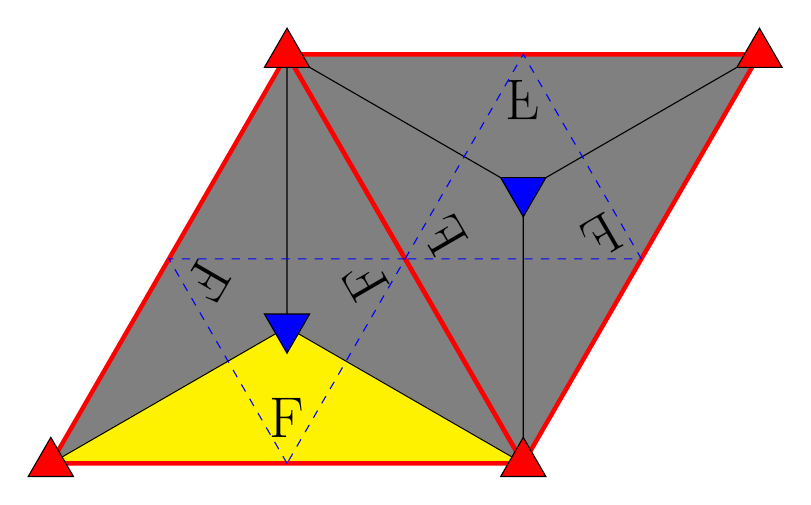
\begin{tikzpicture}
            % Define the lengths of the sides and the angle
            \def\a{3}  % length of side a
            \def\b{3}  % length of side b
            \def\angle{60}  % angle between sides a and b
            \def\s{F} % Label in center of cells

            \def\x{0.5} % Boundary 
            \def\y{0.5} % Boundary
        
            % Calculate the coordinates of the points
            \coordinate (C00) at (0, 0);
            \coordinate (C10) at (\a, 0);
            \coordinate (C11) at ({\a + \b*cos(\angle)}, {\b * sin(\angle)});
            \coordinate (C01) at ({\b * cos(\angle)}, {\b * sin(\angle)});
            \coordinate (C02) at ({2*\b*cos(\angle)}, {2*\b * sin(\angle)});
            \coordinate (C12) at ({\a +2*\b * cos(\angle)}, {2*\b * sin(\angle)});
            \coordinate (C22) at ({2*\a + 2*\b * cos(\angle)}, {2*\b * sin(\angle)});
            \coordinate (C21) at ({2*\a + \b*cos(\angle)}, {\b * sin(\angle)});
            \coordinate (C20) at ({2*\a}, 0);

            \coordinate (A1) at ($(C00)!0.6666!(C11)$);
            \coordinate (A2) at ($(C11)!0.3333!(C22)$);
        
            % Draw the oblique unit cell
            \draw[fill=gray,gray] (C00) -- (C20) -- (C22) -- (C02) -- cycle;
            \draw[fill=yellow,yellow] (C00) -- (A1) -- (C20) -- cycle;
            
            
            
            % Draw chiral center
            \node at ($(C00)!0.5!(C20)!0.3333!(A1)$) {\huge \s};
            \node[rotate=240] at ($(C00)!0.5!(C02)!0.3333!(A1)$) {\huge \s};
            \node[rotate=120] at ($(C20)!0.5!(C02)!0.3333!(A1)$) {\huge \s};
            \node[rotate=300] at ($(C20)!0.5!(C02)!0.3333!(A2)$) {\reflectbox{\huge \s}};
            \node[rotate=30] at ($(C20)!0.5!(C22)!0.3333!(A2)$) {\reflectbox{\huge \s}};
            \node[rotate=180] at ($(C02)!0.5!(C22)!0.3333!(A2)$) {\reflectbox{\huge \s}};

            % Draw mirrow lines
            \draw[ultra thick,red] (C00) -- (C02) -- (C20) -- cycle;
            \draw[ultra thick,red] (C02) -- (C22) -- (C20) -- cycle;
            \draw[thin] (C00) -- (A1) -- (C02) -- (A2) -- (C22);
            \draw[thin] (A1) -- (C20) -- (A2);
            \draw[dashed,blue] (C10) -- (C01) -- (C11) -- cycle;
            \draw[dashed,blue] (C11) -- (C12) -- (C21) -- cycle;
            

            % Draw node rotations symbols
            \draw (C00)  node[regular polygon, regular polygon sides=3, draw, fill=red, minimum size=0.5cm] {};
            \draw (C02)  node[regular polygon, regular polygon sides=3, draw, fill=red, minimum size=0.5cm] {};
            \draw (C22)  node[regular polygon, regular polygon sides=3, draw, fill=red, minimum size=0.5cm] {};
            \draw (C20)  node[regular polygon, regular polygon sides=3, draw, fill=red, minimum size=0.5cm] {};

            \draw (A1)  node[rotate = 180,regular polygon, regular polygon sides=3, draw, fill=blue, minimum size=0.5cm] {};
            \draw (A2)  node[rotate=180, regular polygon, regular polygon sides=3, draw, fill=blue, minimum size=0.5cm] {};

        \end{tikzpicture}
\end{document}}
        \caption{p31m}
    \end{minipage}
    
    \caption{The 17 Wallpaper Groups}
    \label{fig:17-wallpaper-groups}
\end{figure}

\end{document}